\section{Lavoro precedente}


\subsection{Introduzione}

\noindent Per quanto riguarda la valutazione e la predizione delle emissioni questa prima parte del documento si propone di presentare lo stato attuale del lavoro svolto in questo ambito.





\begin{figure}[H]
    \centering
    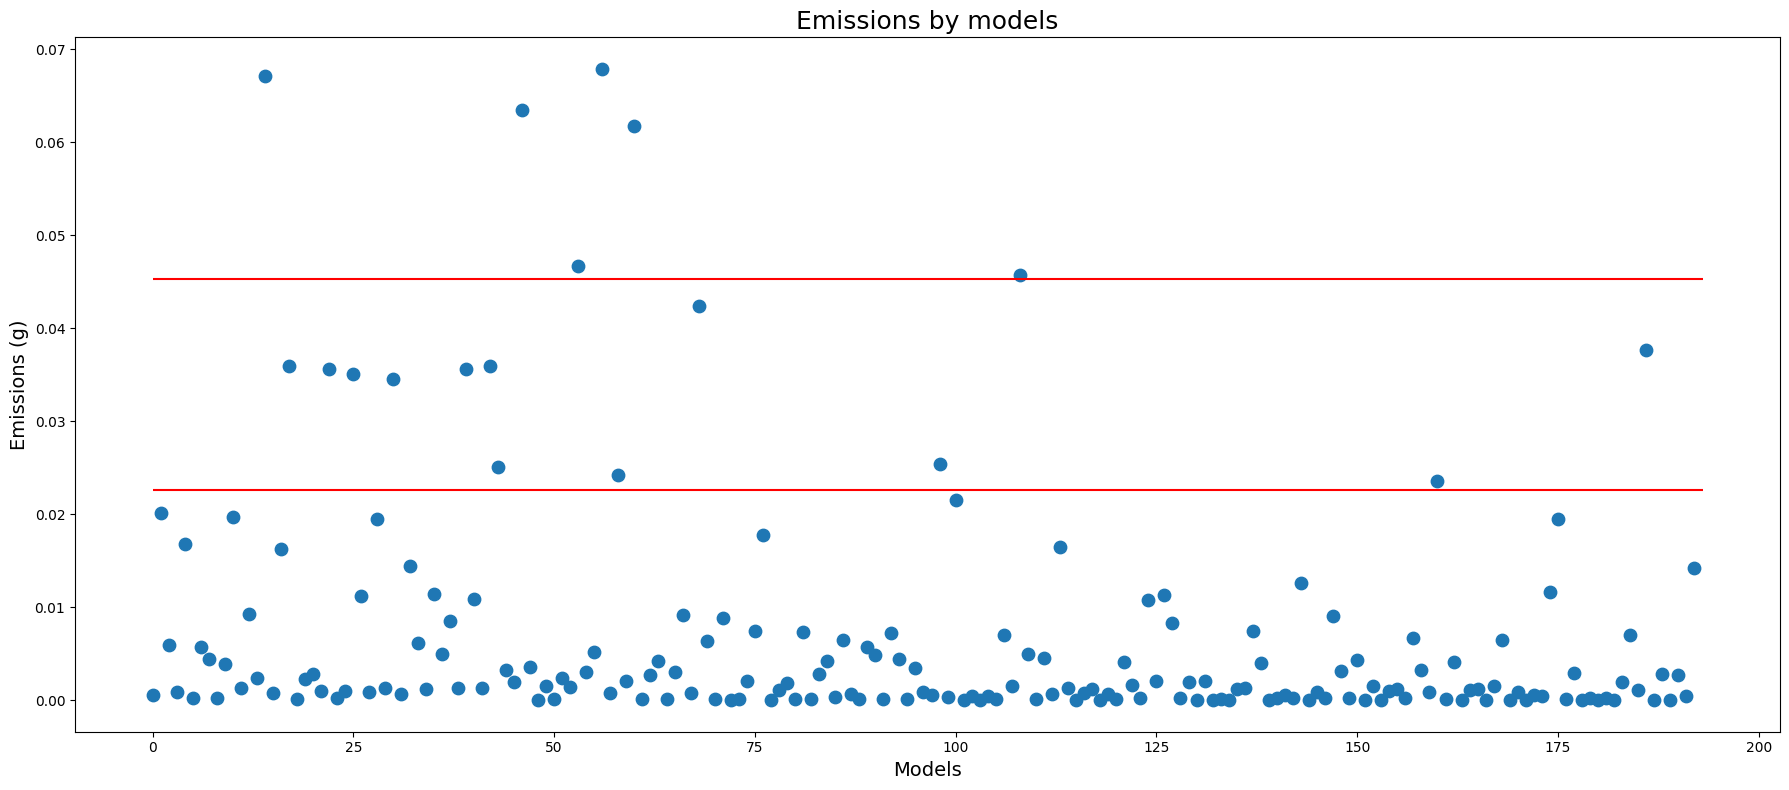
\includegraphics[width=\textwidth]{images/situazione-attuale.png}
    \caption{Emissioni prodotte dai vari modelli}
\end{figure}

\noindent L'esperimento è stato condotto su dataset presenti all'interno della libreria python RecBole\footnote{\href{http://recbole.io}{RecBole}}{}, una libreria open-source che offre un'implementazione di modelli di raccomandazione. I dataset utilizzati per l'addestramento dei modelli sono:
\begin{itemize}
    \item \textbf{MovieLens-1M}\footnote{\href{https://github.com/RUCAIBox/RecSysDatasets/blob/master/conversion_tools/usage/MovieLens.md}{Dataset MovieLens}}{}
    \item \textbf{Amazon\_Book\_60core\_kg} \footnote{\href{https://github.com/RUCAIBox/RecSysDatasets/blob/master/conversion_tools/usage/Amazon-book-KG.md}{Dataset Amazon\_Book\_60core\_kg}}{}
    \item \textbf{Mind}\footnote{\href{https://github.com/RUCAIBox/RecSysDatasets/blob/master/conversion_tools/usage/MIND.md}{Dataset MIND}}{}
\end{itemize}



\subsection {Dataset del regressore}
In questo paragrafo si analizza il dataset utilizzato e come questo è stato trattato per l'addestramento dei modelli. Inoltre, si descrivono le feature di input e output del modello.
Nel dataset sono presenti 201 righe (dunque 201 esperimenti distinti).

\noindent Il dataset nella sua totalità è composto da 13 feature di input e una feature di output.
\subsection{Descrizione della feature di output}
La feature di output \textit{emissions} rappresenta le emissioni di CO$_2$eq prodotte dalla macchina durante l'addestramento del modello.
\subsubsection{Descrizione delle feature di input}
Le feature di input possono essere suddivise in 4 categorie:
\begin{itemize}
    \item \textbf{Feature relative al dataset}, quali \textit{n\_users}, \textit{n\_items}, \textit{n\_inter}, \textit{sparsity}
    \item \textbf{Feature relative al knowledge graph}, quali \textit{kg\_entities}, \textit{kg\_relations}, \textit{kg\_triples}, \textit{kg\_items}
    \item \textbf{Feature relative all'hardware utilizzato per l'addestramento}, quali \textit{cpu\_cores}, \textit{ram\_size}, \textit{is\_gpu}
    \item \textbf{Feature relative al modello}, quali \textit{model\_name}, \textit{model\_type}
\end{itemize}
\begin{center}
\begin{table}[H]
    \centering
    \begin{tabularx}{\textwidth}{|c|X|}
        \hline
        \textbf{Feature} & \textbf{Descrizione} \\
        \hline
        n\_users & Numero di utenti presenti nel dataset \\
        \hline
        n\_items & Numero di items presenti nel dataset \\
        \hline
        n\_inter & Numero di interazioni nel dataset. Per interazione si intendono le varie interazioni (valutazioni) tra gli utenti nel dataset e gli item nel dataset \\
        \hline
        sparsity & Sparsità del dataset. La sparsità indica la percentuale di valori mancanti nel dataset (quindi mancanza di interazione tra utenti e item)\\
        \hline
        kg\_entities & Numero di entità nel knowledge graph. Un'entità è un oggetto distintivo o un concetto unico all'interno del Knowledge Graph \\
        \hline
        kg\_relations & Numero di relazioni nel knowledge graph. Le relazioni rappresentano i legami o collegamenti tra le entità all'interno del Knowledge Graph. Sono spesso definite dai predicati nelle triple \\
        \hline
        kg\_triples & Numero di triple nel knowledge graph. Una triple è una struttura dati fondamentale nel Knowledge Graph che consiste in tre parti: soggetto, predicato e oggetto. Queste triple rappresentano le relazioni tra le entità \\
        \hline
        kg\_items & Numero di items nel knowledge graph. Gli "Items" nel contesto del Knowledge Graph sono gli oggetti specifici o le entità che sono inclusi nel grafo \\
        \hline
        cpu\_cores & Numero di core della CPU \\
        \hline
        ram\_size & Dimensione della RAM \\
        \hline
        is\_gpu & Booleano che indica se la macchina ha usato una GPU per l'addestramento \\
        \hline
        model\_name & Nome del modello \\
        \hline
        model\_type & Tipo del modello \\
        \hline
    \end{tabularx}
    \caption{Descrizione delle feature di input}
\end{table}
\end{center}

\noindent Per quanto riguarda la feature \textit{model\_type} abbiamo i seguenti valori:
\begin{itemize}
    \item \textbf{General}: Modelli che si basano su tecniche tradizionali
    \item \textbf{Knowledge}: Modelli che incorporano conoscenza esterna (knowledge graph) per migliorare le raccomandazioni
\end{itemize}

Per quanto riguarda la feature \textit{model\_name} abbiamo i seguenti valori:
\begin{itemize}
    \item \textbf{BPR} \cite{BPR}: General
    \item \textbf{CDAE} \cite{CDAE}: General
    \item \textbf{CFKG} \cite{CFKG}: Knowledge
    \item \textbf{CKE} \cite{CKE}: Knowledge
    \item \textbf{DGCF} \cite{DGCF}: Knowledge
    \item \textbf{DMF} \cite{DMF}: General
    \item \textbf{DiffRec} \cite{DiffRec}: General
    \item \textbf{ENMF} \cite{ENMF}: General 
    \item \textbf{FISM} \cite{FISM}: General
    \item \textbf{GCMC} \cite{GCMC}: General
    \item \textbf{ItemKNN} \cite{ItemKNN}: General
    \item \textbf{KGCN} \cite{KGCN}: Knowledge
    \item \textbf{KGIN}: \cite{KGIN} Knowledge
    \item \textbf{KGNNLS} \cite{KGNNLS}: Knowledge
    \item \textbf{KTUP} \cite{KTUP}: Knowledge
    \item \textbf{LDiffRec} \cite{LDiffRec}: General
    \item \textbf{LINE} \cite{LINE}: General
    \item \textbf{LightGCN} \cite{LightGCN}: General
    \item \textbf{MKR} \cite{MKR}: Knowledge
    \item \textbf{MacridVAE} \cite{MacridVAE}: General
    \item \textbf{MultiDAE} \cite{MultiDAE}: General
    \item \textbf{MultiVAE} \cite{MultiVAE}: General
    \item \textbf{NCEPLRec} \cite{NCEPLRec}: General
    \item \textbf{NCL} \cite{NCL}: General
    \item \textbf{NGCF} \cite{NGCF}: General
    \item \textbf{NeuMF} \cite{NeuMF}: General
    \item \textbf{Pop}: General
    \item \textbf{Random}: General
    \item \textbf{RecVAE} \cite{RecVAE}: General
    \item \textbf{RippleNet} \cite{RippleNet}: Knowledge
    \item \textbf{SGL} \cite{SGL}: General
    \item \textbf{SLIMElastic} \cite{SLIMElastic}: General
    \item \textbf{SimpleX} \cite{SimpleX}: General
    \item \textbf{SpectralCF} \cite{SpectralCF}: General
    \item \textbf{EASE} \cite{EASE}: General
    \item \textbf{NAIS} \cite{NAIS}: General
    \item \textbf{ADMMSLIM} \cite{ADMMSLIM}: General
    \item \textbf{ConvNCF} \cite{ConvNCF}: General
    \item \textbf{NNCF} \cite{NNCF}: General
\end{itemize}

Altri valori unici presenti per le varie feature di input sono:
\begin{itemize}
    \item \textbf{n\_users}: [22155, 23679, 6040]
    \item \textbf{n\_items}: [54458, 4414, 3706]
    \item \textbf{n\_inter}: [1465871, 1048575, 1000209]
    \item \textbf{sparsity}: [0.99878504, 0.98996762, 0.95531637]
    \item \textbf{kg\_entities}: [26315, 0, 79347]
    \item \textbf{kg\_relations}: [16, 0, 49]
    \item \textbf{kg\_triples}: [96476, 0, 385923]
    \item \textbf{kg\_items}: [11446, 0, 3655]
    \item \textbf{cpu\_cores}: [12, 4]
    \item \textbf{ram\_size}: [64, 16, 27.40581512]
    \item \textbf{is\_gpu}: [1, 0]
\end{itemize}
\subsubsection{Pre-Processing}

Per poter sfruttare le feature di input per l'addestramento del modello, è stato necessario effettuare un pre-processing. Le feature \textit{model\_name} e \textit{model\_type} sono state trasformate in variabili numeriche. In particolare il valore \textit{general} è stato trasformato in 0 e il valore \textit{knowledge} è stato trasformato in 1.
Per quanto riguarda la feature \textit{model\_name}, ogni valore è stato trasformato in un numero intero univoco. In questo modo, il modello di regressione può sfruttare queste feature per l'addestramento.
Prima di cominciare con l'addestramento dei modelli la feature di output è stata separata dalle feature di input. I dati sono poi stati suddivisi rispettivamente in training set e test set. In particolare il 70\% dei dati è stato usato per l'addestramento, mentre il 30\% è stato usato per la valutazione. Inoltre, mediante il \textit{random\_state}=2, è garantita la riproducibilità dell'esperimento.

